%!TEX root=../../main.tex

\section{Backend - REST-Schnittstelle und Infrastruktur}
\label{chap:backendsota}
	\subsection{Einleitung}
	Das \textit{Backend} besteht aus mehreren Komponenten. Einerseits soll eine gewisse System-Infrastruktur aufgebaut werden, um das \textit{\gls{webinterface}} und die \textit{REST}-Schnittstelle bereitzustellen. Andererseits muss die Anwendung selbst entwickelt werden. Diese besteht aus mehreren Teilen. Darunter fällt die \textit{REST}-Schnittstelle, inklusive der implementierten \textit{Endpoints}, Schnittstellen zu diversen Diensten, wie dem \textit{TGM}-\textit{LDAP} \textit{Server}, zur Datenbank und zu \textit{WebUntis}, aber auch die allgemeine Funktionalität der Anwendung, unter anderem das Erstellen von \textit{PDF}-Dateien. Für die Verbindung zu den Schnittstellen sowie zur Implementierung der geforderten Funktionalität werden diverse  \textit{\gls{tpp}} genutzt werden. Die folgende Grafik gibt einen Überblick hinter der Infrastruktur und den verwendeten Diensten:
	\begin{figure}[H]
		\centering
		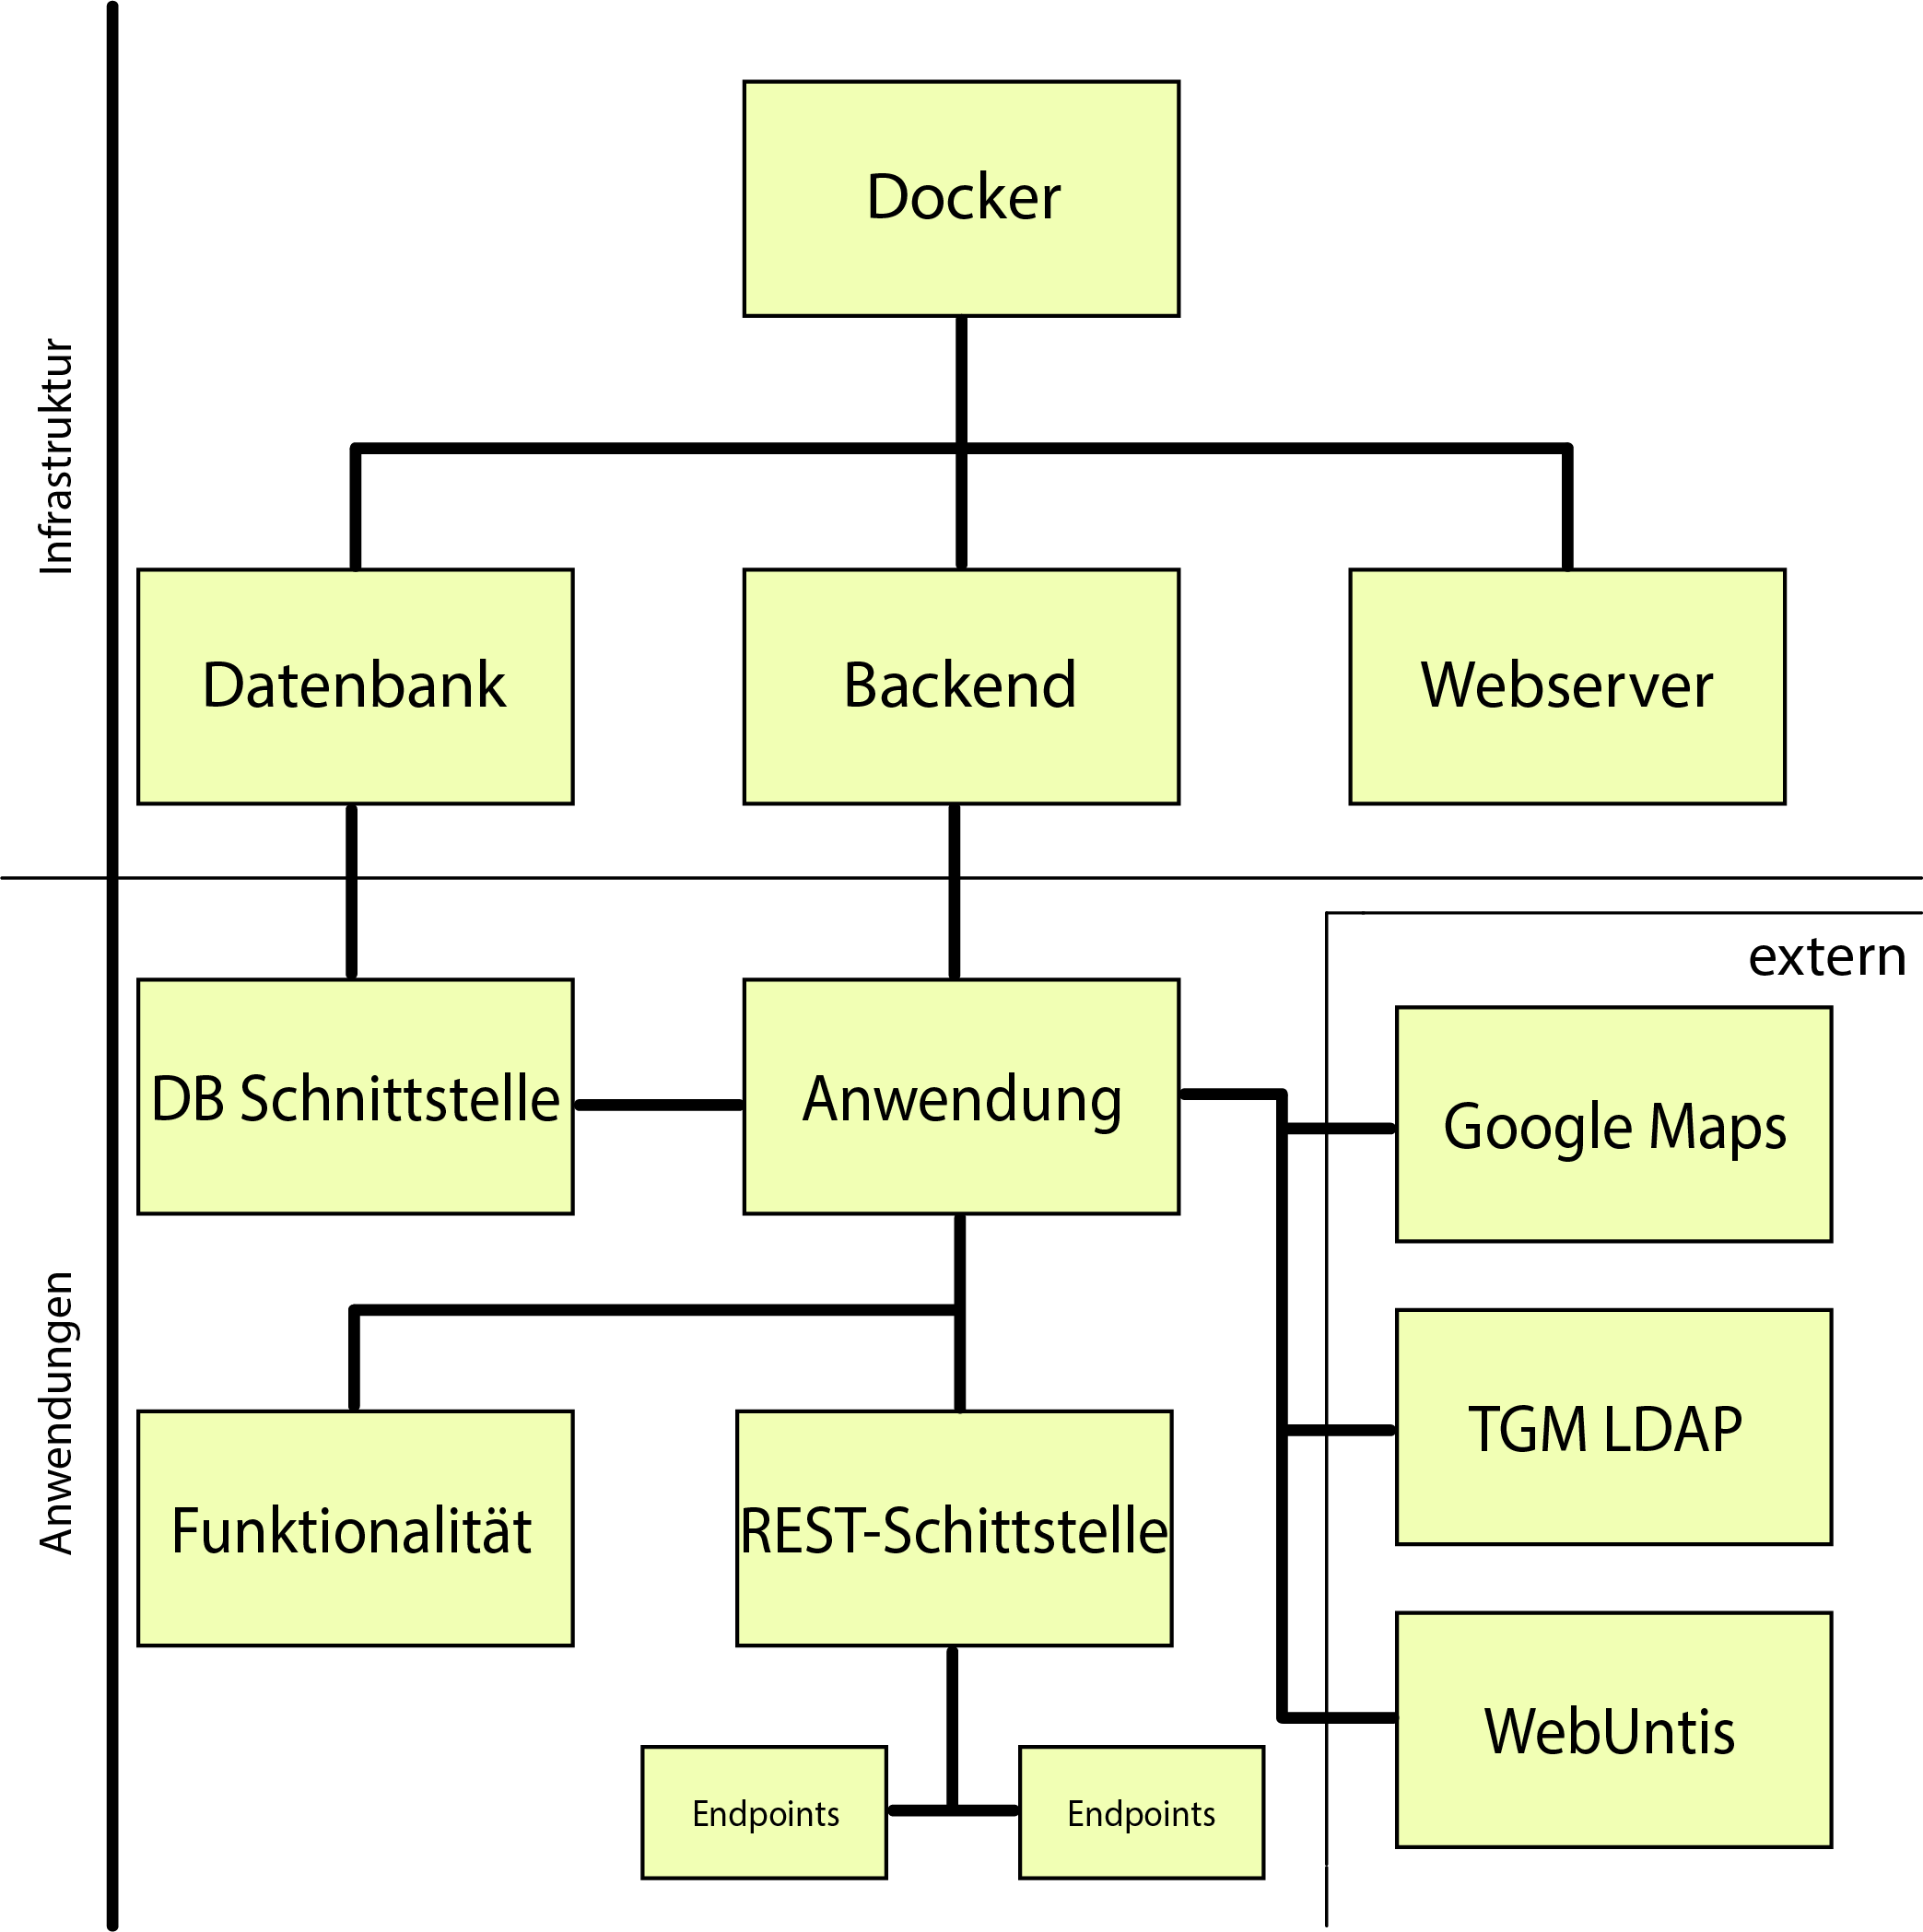
\includegraphics[width=0.8\linewidth]{images/uebersicht}
		\caption[Übersicht über die Komponenten]{Übersicht über die verschiedenen Komponenten der Infrastruktur und der Anwendung}
		\label{fig:uebersicht}
	\end{figure}
	
	\newpage
	In den folgenden Kapiteln werden die aktuell verfügbaren Technologien, welche für die Umsetzung im \textit{Backendbereich} in Frage kommen, beschrieben und gegebenenfalls - sofern mehrere sinnvolle Kandidaten vorhanden sind - auch verglichen. Auf einen detaillierten Vergleich jeglicher verwendbaren \textit{Third Party Packages}, welche dazu genutzt werden könnten, um die Funktionalität im Backend zu implementieren, wird auf Grund der extrem hohen Anzahl im Sinne der Übersichtlichkeit verzichtet. Unter die benutzten Bibliotheken, fallen jedenfalls Module wie \enquote{\textit{maroto}} (zum Erstellen von \textit{PDF}-Dateien \cite{maroto}), \enquote{\textit{excelize}} (zum Erstellen von \textit{Excel}-Dateien \cite{excelize}) und \enquote{\textit{jwt-go}} (zum Erstellen von \textit{\Gls{jwt}} \cite{jwt-go}) 
	\subsection{Docker}
	Um die Infrastruktur des Projektes einfach aufbauen zu können, wird \textit{\Gls{docker}} genutzt. Da es sich hier um eine komplex strukturierte Infrastruktur handelt, wird zusätzlich das Werkzeug \textit{\Gls{dcompose}} genutzt. Mit \textit{Docker Compose} kann eine Infrastruktur aufgebaut werden, die der \hyperref[fig:uebersicht]{Abbildung 5.2} entspricht. Für diese sind folgende \textit{Container} vorgesehen, die in den nächsten Kapiteln noch im Detail beschrieben werden.
		\subsubsection{Datenbank}
		\label{sec:db}
		Um die Daten, die durch \textit{Refundable} erhoben und generiert werden, zu speichern, wird eine \gls{db} benötigt. Auf Grund der Daten, welche sich durch unterschiedliche Datenstrukturen auszeichnen, ist der Einsatz einer \gls{relDb} nicht sinnvoll. Stattdessen empfiehlt sich die Verwendung einer \gls{nosqlDb}.
		Standardmäßig wird zwischen 4 verschiedenen Typen von \textit{NoSQL} Datenbanken unterschieden, welche jeweils nur in ihrem eigenen \textit{Use Cases} sinnvoll anwendbar sind \cite{nosqltypes}:
		\begin{itemize}
			\item \textit{Key}-\textit{Value} Datenbank
			\item spaltenorientierte Datenbank
			\item graphenorientierte Datenbank
			\item dokumentenorientierte Datenbank
		\end{itemize}
		\captionof{listing}{\textit{NoSQL} Datenbank-Typen}
		\label{code:nosqltypes}~\\	
		Bei \textit{Key}-\textit{Value} Datenbanken wird einem Schlüssel ein Wert hinterlegt. Dieser Wert ist dann jederzeit über den Schlüssel in der Datenbank abrufbar. Für unseren \textit{Use Case} ist dieses System nicht sinnvoll anzuwenden, da die von uns benutzten Daten hierfür zu komplex im Aufbau sind.~\\
		Bei spaltenorientierten Datenbanken werden Daten vorrangig über ihre Spalten (statt wie bei relationalen \gls{db}s in Zeilen) analysiert. Dies ermöglicht die einfache Umsetzung statistischer Methoden auf Basis der Spalten. Da jedoch wieder eine Tabelle als Grundstruktur vorliegt, ist dieser Typ von Datenbank nicht sinnvoll anwendbar für \textit{Refundable}.~\\
		Bei graphenorientierten Daten wird die Beziehung zwischen einzelnen Elementen hervorgehoben. Daten werden hier in Knoten gespeichert, welche zu anderen verbunden werden können. Die primären Elemente sind hierbei die Beziehungen, anstatt der Daten selbst. Da die Daten von \textit{Refundable} nicht über starke Beziehungen charakterisiert sind, ist auch dieser Datenbank-Typ nicht sinnvoll zu benutzen.~\\		
		Zuletzt bei dokumentenorientierten Datenbanken unterliegt jeder Datensatz in einem eigenen Dokument, welches in \textit{\Gls{json}}, \textit{\Gls{yaml}}, \textit{\Gls{xml}} oder ähnlichen Datenformaten gespeichert wird. Dadurch ist auch eine jeweils von einander unabhängige Datenstruktur möglich. Auf Grund der Flexibilität bei Datenstrukturen ist eine dokumentenorientierte Datenbank eindeutig sinnvoll zu verwenden.~\\
		Als \gls{dbms} kommt bei dieser Auswahl einige Software in Frage. Die am meisten verbreitete Software hier ist \textit{MongoDB} und \textit{CouchDB} \cite{mongo}. Wo \textit{MongoDB} auf strenge \gls{konsistenz} setzt, setzt \textit{CouchDB} auf hohe \gls{verfugbarkeit}. Da in unserem Projekt Konsistenz wichtiger ist als Verfügbarkeit wird \textit{MongoDB} in einem Container als Datenbankmanagementsystem verwendet.
		
		\subsubsection{Backend-Container}
		
		Ebenfalls wird ein \textit{Container}, also eine Umgebung, in dem das \textit{Backend} laufen kann, erstellt. Dieser wird direkt zu den anderen \textit{Containern} hinzugefügt, damit dieser über ein \textit{Docker}-Netzwerk mit den anderen \textit{Containern} kommunizieren kann.~\\
		Um diesen \textit{Container} zu realisieren wird als Basis ein \enquote{\textit{golang}}-\textit{Image} genutzt \cite{golang}. Dieses stellt eine sehr sparsame Linux-Instanz dar, welche mit einer \enquote{\textit{golang}}-Umgebung ausgestattet ist. Um diesen \textit{Container} noch entsprechend anzupassen, wird ein entsprechendes \textit{Docker}-\textit{Image} über ein \textit{Dockerfile} gebaut.
		
		\subsubsection{Webserver}
		
		Als \textit{Webserver} wird ein \textit{Apache2} \textit{Server} genutzt \cite{apache}. Der Service stellt hierbei das \textit{Webinterface} (\textit{Frontend}) im Internet zur Verfügung. Dieser \textit{Container} ruft automatisch das \textit{Frontend} auf und kopiert es in seine Umgebung. Ebenfalls muss der \textit{Container} Zugriff auf Zertifikaten bekommen, um einen sicheren Zugriff über \textit{\gls{https}} gewährleisten zu können.
				
	\subsection{Deployment}
	
	Das \textit{Deployment} soll automatisch geschehen. Um dies einfach zu ermöglichen, werden die oben zuvor beschriebenen \textit{Docker}-\textit{Container}, \textit{GitHub} und ein Skript, welches die Schritte ausführt, genutzt. Das Skript ist hier der Hauptbaustein, welcher den Vorgang startet und steuert. Zusätzlich zum Installationsvorgang, soll das Skript auch die weitere Steuerung der Software, also starten, stoppen, updaten, cleanen und deinstallieren, beinhalten.~\\
	Das Skript liegt in einem eigenem \textit{Install}-\textit{\Gls{repo}}, in welchem sonst keine weiteren Dateien liegen. Dadurch kann es einfach geklont und direkt installiert werden; die restlichen Installations-Schritte werden automatisch erledigt.~\\
	Da das \textit{Deployment} auf einer \textit{Linux}-Maschine ermöglicht werden soll, wird \textit{\Gls{bash}} als Standard-Skriptsprache benutzt. Zur Verteilung des Scripts wird, wie erwähnt, \textit{\Gls{git}} mit dem \textit{Online Repository-Hosting Service \Gls{github}} verwendet.
	\subsection{REST-Schnittstelle}
	Bei einer \textit{REST}-Schnittstelle handelt es sich um einen bestimmten Aufbau einer Softwareschnittstelle bei verteilten Systemen \cite{Patni2017}. Das hierbei angewendete Prinzip nennt sich \enquote{\textit{Representational State Transfer}} (kurz \textit{REST}). Es zeichnet sich durch folgende Eigenschaften aus:
	\begin{itemize}
		\item \textbf{Client-Server}, wobei es um eine strikte Trennung zwischen dem \textit{Client} (dem \textit{REST}-\textit{Client}) und dem \textit{Server} (der \textit{REST}-Schnittstelle, als \textit{Webservice}) geht
		\item \textbf{Stateless}, wobei es um die Zustandslosigkeit des \textit{Servers} geht. Das heißt, dass der Server sich keinerlei Zustände der \textit{Clients} merkt.
		\item \textbf{Caching}: Der \textit{Server} speichert die \textit{Responses} zwischen. Dadurch kann die Latenzzeit minimiert werden, da Daten öfters zurückgegeben werden, anstatt sie jedes Mal erneut berechnen zu müssen.
		\item \textbf{Einheitliche Schnittstelle} bedeutet, dass die Schnittstelle ein einheitliches Datenformat verwendet, um via \textit{HTTP} über \textit{CRUD}-Methoden (\textit{Create}, \textit{Read}, \textit{Update}, \textit{Delete}) zu kommunizieren.
		\item \textbf{Layer-System} bedeutet, dass die Schnittstelle, als \textit{Webservice} so designt wird, dass auch weitere Schichten, wie \textit{Gateways} und \textit{Proxies}, transparent dazwischen aufgebaut werden können.
		\item \textbf{Code-on-demand} (optional): Hierbei besteht die Möglichkeit ausführbaren \textit{Code} an die \textit{Clients} zu schicken, sodass diese den dann ausführen können.
	\end{itemize}
	\captionof{listing}{Prinzipien des \textit{Representation State Transfer}}
	\label{code:rest}
		\subsubsection{Java und Spring}
		\textit{Java} ist eine der bekanntesten Programmiersprachen. Sie zeichnet sich durch Plattform-Unabhängigkeit aus \cite{jdkDocs}. Um dies zu erreichen, wird \textit{Bytecode} von einem eigenem Programm, der \textit{Java Virtual Machine}, interpretiert. \textit{Java} arbeitet objektorientiert und ist statisch typisiert. Dies bedeutet, dass bereits vor dem Ausführen die Datentypen definiert sind. \textit{Java} unterstützt auch \textit{Multithreading}. Um einfach eine \textit{REST}-Schnittstelle in \textit{Java} bauen zu können, wird \textit{Spring Boot} genutzt \cite{springDocs}. Die Verwendung von \textit{Spring} ermöglicht \textit{Webapps}, \textit{Tasks} oder \textit{Microservices} einfacher umzusetzen. Prinzipiell arbeitet \textit{Spring} asynchron und flexibel, sodass es einfach zu skalieren ist. 
		
		\subsubsection{Python und Flask}
		Um mit \textit{Python} eine \textit{REST}-Schnittstelle zu realisieren muss auf das \textit{Package} (\textit{Framework}) \textit{Python} \textit{Flask} zurückgegriffen werden \cite{flaskDocs}. \textit{Flask} wird hierbei dazu genutzt, um den \textit{Webservice} zu bauen. \textit{Python} und \textit{Java} unterscheiden sich prinzipiell sehr. \textit{Python} ist im Gegensatz zu \textit{Java} dynamisch typisiert, dies bedeutet, dass eine Variablendeklaration nicht notwendig ist und der Datentyp einer Variable erst zur Laufzeit klar ist \cite{pythonDocs}. Anders als \textit{Java} setzt \textit{Python} auf \textit{Third-Party Packages}, welche sehr einfach importiert werden können. Durch die große \textit{Community} \textit{Pythons} ist ein Großteil der \textit{Tools}, die man benötigt, meist schon vorprogrammiert und kann einfach importiert werden. Zusätzlich ist der Syntax (speziell was Zeichensetzung anbelangt) einfacher zu verstehen, als jener von \textit{Java}.
		
		\subsubsection{Golang}
		\label{chapter:golanganalyse}
		\textit{Golang} (kurz \textit{Go}) ist eine von \textit{Google} entwickelte und publizierte Programmiersprache \cite{goDocs}. Sie wurde aus der Unzufriedenheit über \textit{Java}, \textit{C++} und \textit{Python} heraus entwickelt, welche am häufigsten bei \textit{Google} eingesetzt wurden. All diese Programmiersprachen haben Nachteile in \textit{Googles} \textit{Business Case}, deswegen wurde \textit{Go} speziell für skalierbare Netzwerkdienste und \textit{Cloud Computing} entwickelt. Aus diesem Grund besitzt \textit{Go} auch eine native Möglichkeit für den einfachen Aufbau von \textit{REST}-Schnittstellen. Da bei der Entwicklung von \textit{Go} speziell aus den Fehlern in Performance und Sprachdesign aus anderen Sprachen gelernt wurde, verbindet \textit{Go} die Vorteile der anderen Sprachen. Darunter fallen die starke und statische Typisierung, Objektorientierung, \textit{Pointer} und eine verbesserte \textit{Compiler}-Effizienz.
		\newpage
		\subsubsection{Vergleich}
		Diese drei Sprachen werden nun in den Aspekten der Performance, dem Sprachdesign, der Komplexität des Aufbaus einer \textit{REST}-Schnittstelle, das Vorhandensein von \textit{Frameworks}, die Erfahrung des Teams und eine vorhandene ausführliche Dokumentation analysiert und verglichen. Hierbei wird auf einer Punkteskala von 0 - 9 bewertet.
		\captionof{table}{Vergleich zwischen Java, Python und Golang}\label{tbl:comparisonlang}
		\begin{table}
			\begin{tabular}{|l|r|r|r|r|r|r|r|}
				\hline
				\multicolumn{1}{|c|}{\textbf{Kriterien}} & \multicolumn{1}{c|}{\textbf{Gewichtung}} & \multicolumn{2}{c|}{\textbf{Java und Spring}} & \multicolumn{2}{c|}{\textbf{Python und Flask}} & \multicolumn{2}{c|}{\textbf{Golang}} \\ \cline{3-8} 
				& \multicolumn{1}{l|}{} & \multicolumn{1}{c|}{Punkte} & \multicolumn{1}{c|}{Wertung} & \multicolumn{1}{c|}{Punkte} & \multicolumn{1}{c|}{Wertung} & \multicolumn{1}{c|}{Punkte} & \multicolumn{1}{c|}{Wertung} \\ \hline
				Performance & 15\% & 6 & 0,9 & 3 & 0,45 & 9 & 1,35 \\ \hline
				Sprachdesign & 25\% & 6 & 1,5 & 4 & 1 & 8 & 2 \\ \hline
				\begin{tabular}[c]{@{}l@{}}Aufbau einer \\ REST-Schnittstelle\end{tabular} & 5\% & 7 & 0,35 & 8 & 0,40 & 9 & 0,45 \\ \hline
				\begin{tabular}[c]{@{}l@{}}Vorhandensein von\\ Frameworks\end{tabular} & 15\% & 7 & 1,05 & 9 & 1,35 & 9 & 1,35 \\ \hline
				\begin{tabular}[c]{@{}l@{}}Erfahrung des \\ Teams\end{tabular} & 20\% & 4 & 0,8 & 3 & 0,6 & 6 & 1,2 \\ \hline
				Dokumentation & 20\% & 8 & 1,6 & 7 & 1,4 & 9 & 1,8 \\ \hline
				\textbf{Summe} & 100\% & \multicolumn{1}{l|}{} & \multicolumn{1}{c|}{\textbf{6,2}} & \multicolumn{1}{c|}{\textbf{}} & \multicolumn{1}{c|}{\textbf{5,2}} & \multicolumn{1}{c|}{\textbf{}} & \multicolumn{1}{c|}{\textbf{8,15}} \\ \hline
			\end{tabular}
		\end{table}
		~\\
		Daraus und aus der durchgeführten Recherche, lässt sich schließen, dass \textit{Golang} sich speziell bei den Punkten Performance und Sprachdesign durchsetzen kann. Ansonsten schneiden die verschiedenen Sprachen inklusive der teilweise benötigten \textit{Frameworks} großteils ähnlich hoch ab. Zusammenfassend eignet sich die Verwendung von \textit{Golang} am Besten als Programmiersprache für unser Projekt, da sie im numerischen Vergleich mit der höchsten Punktezahl abschnitt, aber auch durch die speziellen Hintergründe ihrer Entwicklung genau zu den Voraussetzungen passt.
	\subsection{Kommunikation und Datenformate}
	Wie bereits erwähnt, zeichnen sich \textit{REST}-Schnittstellen unter anderem dadurch aus, dass sie ein einheitliches Datenformat voraussetzen. Aus diesem Grund stellen sich die Fragen: \\~\\
	Welche Datenformate eignen sich für einen konsistenten und performanten Datenaustausch zwischen Datenbank, \textit{REST}-Schnittstelle und \textit{Client}? \\~\\
	Welche Vor- und Nachteile bringen diese im Hinblick auf Performance, Softwarewartung und -evolution?\\~\\
	Um diese Fragen zu beantworten werden in den nächsten Kapiteln entsprechende Datenformate vorgestellt, beschrieben und analysiert.
	
	\newpage
		\label{sec:json}
		\subsubsection{JSON}
		\textit{\Gls{json}} (\textit{JavaScript Object Notation}) ist ein Textformat, welches für die Serialisierung von Daten genutzt werden kann \cite{rfc4627}. 
		Es umfasst 6 Datentypen, davon 4 Primitive und 2 Strukturen:
		\begin{itemize}
			\item \textit{\Gls{string}s}
			\item Zahlen
			\item \textit{\Gls{bool}s}
			\item \textit{\Gls{null}}
			\item \textit{\Gls{array}s}
			\item \Gls{object}e
		\end{itemize}
		\captionof{listing}{\textit{JSON} - Datentypen}
		\label{code:jsontypes}~\\	
		Wie so eine Serialisierung aussieht, wird in folgendem Beispiel ersichtlich: 
		
		\begin{code}{json}
		{
			"classes": [
				{
					"name": "1AHIT",
					"lastYear": false,
					"students": 35,
					"class-rep": "Michaela Musterfrau"
				},
				{
					"name": "5BHIT",
					"lastYear": true,
					"students": 25,
					"class-rep": "Maximilian Frühmann"
				}
			],
			"date": "2021-09-01"
		}
		\end{code}
		\captionof{listing}{\textit{JSON} Beispiel}
		\label{code:json}~\\
		Das in \hyperref[code:json]{Auflistung 5.8} stehende Beispiel stellt ein Objekt mit zwei Feldern dar. Das erste Feld ist ein \enquote{classes}-\textit{Array}, welches verschiedene Schulklassen beinhaltet. Diese Schulklassen haben jeweils einen \textit{String} als Namen, einen \textit{Boolean} als Feld, das angibt, ob es sich um eine Abschlussklasse handelt, die Anzahl der Schüler als Zahl und den Namen des Klassensprechers. Nachdem die Definition des \textit{Arrays} abgeschlossen ist, wird noch ein weiteres Feld im obersten Objekt angegeben, welches das aktuelle Datum als \textit{String} beinhaltet.
		\\~\\
		Der \textit{JSON}-Standard umfasst genaue Regeln, wie mit den Datentypen, speziell mit \textit{Strings} und Zahlen, umzugehen ist \cite{rfc4627}.
		Über einen \textit{JSON}-Generator kann ein \textit{JSON}-Text auf Basis eines Dateninputs generiert werden. Wenn die Daten aus dem \textit{JSON}-Textformat wieder extrahiert werden sollen, spricht man vom \enquote{\textit{parsen}} von Daten.\\
		Jede moderne Programmiersprache hat einen eigenen \textit{JSON}-Parser implementiert oder es ist möglich einen über ein \textit{\Gls{tpp}} zu laden.
		\subsubsection{XML}
		\textit{\Gls{xml}} (\textit{Extensible Markup Language}) ist ein strukturiertes textbasiertes Datenformat \cite{xmlStandard}. Es handelt sich hierbei um eine \textit{Markup}-\textit{Language}. Als Syntax von \textit{XML} werden \textit{Tags} verwendet. Ein <Tag> ist ein Anfangs-\textit{Tag} und ein </Tag> ein End-\textit{Tag}. Ebenfalls können Attribute in einem Anfangs-\textit{Tag} definiert werden (<Tag attribut=\dq wert\dq ). \textit{XML}-Dateien brauchen im Gegensatz zu \textit{JSON}-Texten ein Wurzelelement.
		\begin{code}{xml}
		<school>
			<classes>
				<class lastYear="false" students="35" class-rep="null">1AHIT</class>
				<class lastYear="true" students="25" class-rep="null">5BHIT</class>
			</classes>
			<date>2021-09-01</date>
		</school>
		\end{code}
		\captionof{listing}{\textit{XML} Beispiel}
		\label{code:xml}~\\
		Das Beispiel definiert ein Wurzelelement für die Datenstruktur namens \enquote{school}. Dieses hat ein Kindelement \enquote{classes}. In diesem sind einzelne \enquote{class}-\textit{Tags} mit den nötigen Attributen und dem Namen der Klasse innerhalb der \textit{Tags}. Dies wird als Alternative für die in \textit{XML} nicht vorhandenen \textit{Arrays} genutzt. Zuletzt wird wieder ein untergeordnetes \enquote{date}-Element mit dem aktuellem Datum als Inhalt hinzugefügt.\\~\\
		Das \textit{XML}-Dateiformat kann entweder gültig oder wohlgeformt sein \cite{xmlStandard}. Dies beschreibt die Einhaltung des Syntax und der Regeln des \textit{XML} Standards.\\
		Des Weiteren besteht die Möglichkeit die Struktur von \textit{XML}-Dateien anhand der \textit{XML}-Schema-Sprache oder durch die \textit{Document Type Definition} zu beschreiben. \textit{XML} Dateien brauchen aus diesen Gründen unbedingt einen \textit{Parser} für die Umwandlung.
		
		\newpage
		
		\subsubsection{CSV}
		\textit{CSV} (\textit{Comma-Separated Values}) ist ein Textformat, mit welchem man Tabellen textbasiert darstellen kann \cite{rfc4180}. Hierbei werden Spalten durch \dq , \dq  ~(Beistriche) getrennt und Zeilen durch einen Zeilenumbruch (\textit{CRLF}; \textit{LF}). Die erste Zeile repräsentiert die Namen der Spalten. Eine Beschreibung einer Tabelle mit \textit{CSV} sieht wie folgt aus:
		\begin{code}{python}
			Class,lastYear,students,class-rep
			1AHIT,false,35,null
			5BHIT,true,25,null
		\end{code}
		\captionof{listing}{\textit{CSV} Beispiel}
		\label{code:csv}~\\
		Im Beispiel werden die beiden Klassen als zwei Datensätze in einer Tabelle aufgelistet. Auf Grund der Struktur von \textit{CSV} ist es nur möglich den \textit{Array}-Teil des Objektes darzustellen. Ansonsten ist der \textit{CSV}-Standard recht simpel gehalten. Der letzte Punkt auf den der Standard hierbei eingeht ist, dass "-Zeichen um die Daten gesetzt werden können \cite{rfc4180}. Sollten, diese nicht geschlossen werden kann es jedoch zu unvorhersehbaren Verhalten kommen.
		\subsubsection{Vergleich}
		Ein Vergleich zwischen den Datenformaten \textit{JSON}, \textit{XML} und \textit{CSV} ist auf dem ersten Blick nicht zielführend. Wie aus den einzelnen Beschreibungen der Technologien oben entnommen werden kann, handelt es sich beim \textit{CSV}-Format um Tabellen. Bereits bei der \hyperref[sec:db]{Wahl der dokumentenorientierten Datenbank \textit{MongoDB}} war der Hintergedanke relationale Datenbanken und ihrer Speicherstruktur, Tabellen, weitestmöglich zu vermeiden. 
		
		Wenn man sich nun auch das \textit{CSV} Format und speziell das \hyperref[code:csv]{Beispiel} anschaut, merkt man, dass die Umwandlung des ursprünglichen Objektes nur indirekt möglich war und als Auflistung der Klassen endete. Das Resultat ist, dass Objekte zu \textit{CSV}-Tabellen mit vielen Spalten und einer Zeile werden und \textit{Arrays} zu Tabellen mit wenigen Spalten und vielen Zeilen. Eine Darstellung beider Datentypen in einer Tabelle ist nicht möglich. Dies disqualifiziert \textit{CSV} für den Einsatz als Datenformat im Projekt.
		
		Vergleicht man nun \textit{JSON} und \textit{XML} so scheinen diese erst ähnlich. Jedoch besteht bei \textit{XML} keine Möglichkeit \textit{Arrays} zu definieren. Des Weiteren wird \textit{XML} nicht nur als Datenformat zur Kommunikation genutzt, sondern hat noch weitere Nutzen als \textit{Markup Language}. Demnach ist \textit{XML} sehr überladen, speziell deswegen weil es einen eigenen speziellen \textit{XML}-\textit{Parser} braucht.
		
		Auch \textit{JSON} braucht einen sogenannten \textit{Parser}, jedoch handelt es sich hierbei nur um das Einlesen des \textit{JSON}-Textes und dem Generieren des Objekts. Eine Validierung wie in \textit{XML} bleibt aus. Zuletzt ist \textit{JSON} nicht nur schneller, sondern auch effizienter was den Verbrauch an \textit{CPU}-Leistung und an Arbeitsspeicher angeht \cite{Nurseitov}.
		
		Aus diesen Gründen wird \textit{JSON} als Datenformat zur Kommunikation zwischen den einzelnen Komponenten \textit{Refundables} genutzt werden.